\documentclass{beamer}
% Packages

% Sets

% Formal statements


\title{Diseño y análisis de algoritmos\\ ISIS1105}
\subtitle{Dynamic programming}
\author{Daniel R. Barrero R.}
\date{\today}

\begin{document}
\frame{\titlepage}

%

\begin{frame}{Making change}
	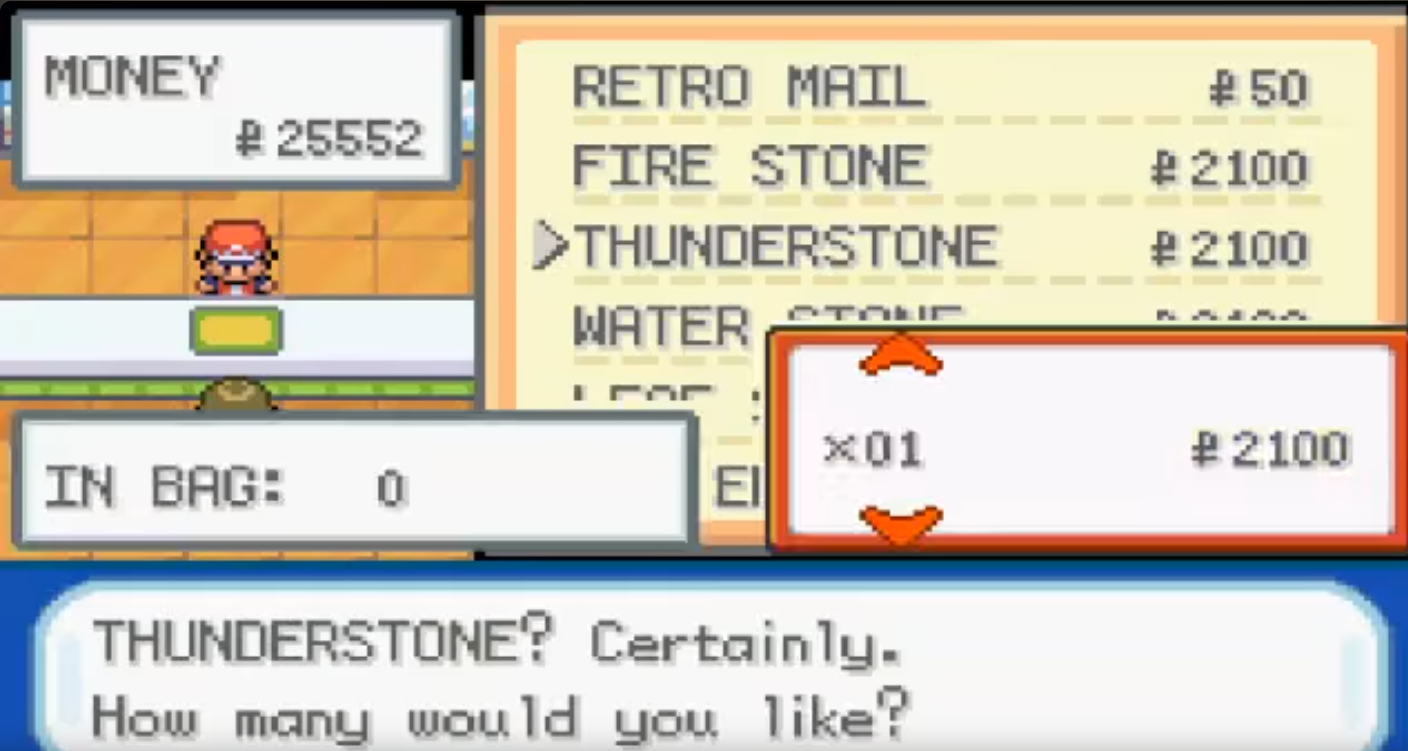
\includegraphics[width=0.5\textwidth]{pokeshopping.png}

	\bigskip
	Let $\mathcal{V}= (v_n, v_{n-1}, \ldots, v_1)$ be a decreasing sequence of
	positive integers, such as $\mathcal{V}_{EEUU}= (50,25,10,5,1)$. The
	\emph{change-making problem} consists of expressing a monetary value
	$N \in \Zpos$ using the least amount of coins $v_i$.\pause
	\ More formally, find
	$a_1, \ldots, a_{n-1}, a_n$ such that
	\[
		\begin{cases}
			N = \sum_{i= 1}^n a_i v_i\\
			\sum_{i= 1}^n a_i = \min \{\sum_{i= 1}^n b_i | b_i \in \NN \land N = \sum_{i= 1}^n b_iv_i\}
		\end{cases}
	\]
\end{frame}

%

\begin{frame}{Making change - greedy}
	A reasonable approach would be to use the largest value first, then the
	second largest, and so on. This is called the \emph{greedy} approach.

	\begin{exl}
		For the coin system $\mathcal{V}_{EEUU} = (50,25,10,5,1)$ the value
		88 is composed as
		\[
			88 = 1*50 + 1*25 + 1*10 + 3*1,
		\]
		using a total of 6 coins.
	\end{exl}
\end{frame}

%

\begin{frame}{Making change - greedy}
	\lstinputlisting[language=Java, firstline=8, lastline=25]{Aula08.java}
\end{frame}

%

\begin{frame}{Making change - greedy gone wrong}
	However, there might be situations where the greedy algorithm fails to
	compose the value using the minimum number of coins. This can happen for
	``bad'' coin systems (\emph{which?!}) or when a ``nice'' coin system is in
	short supply of some denominations.

	\begin{exl}
		Suppose a person using the EEUU system lacks coins of value 5. If
		he or she uses the greedy algorithm to compose the value 30, the
		result will be
		\[
			30 = 1*25 + 5*1,
		\]
		using a total of 6 coins.\pause

		\bigskip
		But we have $\mathcal{V}_{EEUU}' =
		(50,25,10,1)$, so $30 = 3*10$ is possible!
	\end{exl}
\end{frame}

%

\begin{frame}{Quiz \pause - Mentiras! jajajaja}
\end{frame}

%

\begin{frame}{Quiz - Mentiras! jajajaja}
	\begin{exr}
		Find three values of $N$ for which the greedy algorithm fails to
		compose them with minimum number of coins in the system $(5,4,1)$.
	\end{exr}
\end{frame}

%

\begin{frame}{Making change - DP}
	Suppose we want to compose the value 8 \textrm{in} the system with values
	5, 4 and 1.\pause

	\bigskip
	Let's order the denominations from smallest to largest:
	\[
		(v_1, v_2, v_3) = (1, 4, 5)
	\]
	And fill the table \textbf{memo} so that \textbf{memo[i,j]} is the number
	of coins required to compose the value \textbf{j} using the first \textbf{i}
	coins.\pause

	\bigskip
	\begin{tabular}{|| l|c|c|c|c|c|c|c|c ||}\hline
		\textbf{j} & 1 & 2 & 3 & 4 & 5 & 6 & 7 & 8\\\hline
		\textbf{i} & x & x & x & x & x & x & x & x \\\hline\pause
		1          & 1 & 2 & 3 & 4 & 5 & 6 & 7 & 8\\\hline\pause
		2          & 1 & 2 & 3 & 1 & 2 & 3 & 4 & 2\\\hline\pause
		3          & 1 & 2 & 3 & 1 & 1 & 2 & 3 & 2\\\hline
	\end{tabular}
\end{frame}

%

\begin{frame}{Making change - DP}
	\lstinputlisting[language=Java, firstline=31, lastline=44]{Aula08.java}
\end{frame}

%

\begin{frame}{Knapsack}
	
\includegraphics[width=0.25\textwidth]{pokebag.png}
	\hspace{1cm}
	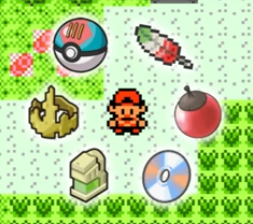
\includegraphics[width=0.25\textwidth]{pokeitems.png}

	\bigskip
	Suppose we have $n$ items, each having weight $w_i$ and value $v_i$. The
	\textbf{knapsack problem} consists of filling a knapsack (\emph{esp. morral})
	of maximum weight capacity $W$ such that the value carried in the bag is
	maximum.
\end{frame}

%

\begin{frame}{Knapsack}
	Namely, we want to

	\bigskip
	\begin{quote}
		maximize $\sum_{i= 1}^n x_iv_i$ 
	\end{quote}
	
	\begin{quote}
		subject to $\sum_{i= 1}^n x_iw_i \leq W$
	\end{quote}
	where $x_i \in \{0,1\}$. \pause

	\begin{exl}
		Suppose we have the (\emph{weight, value}) pairs
		\[
			\begin{array}{lll}
				(7, 28), & (6, 22), & (5, 18),\\
				(2, 6), & (3, 7), & (1, 1).
			\end{array}
		\] \pause
		How can we fill the knapsack via a greedy method versus a dynamic
		programming method?
	\end{exl}
\end{frame}

%

\begin{frame}{Knapsack - greedy}
	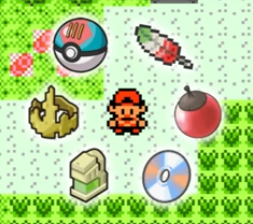
\includegraphics[width=0.25\textwidth]{pokeitems.png}
		\[
			\begin{array}{lll}
				(7, 28), & (6, 22), & (5, 18),\\
				(2, 6), & (3, 7), & (1, 1).
			\end{array}
		\]
\end{frame}

%

\begin{frame}{Knapsack - greedy}
	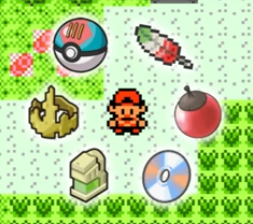
\includegraphics[width=0.25\textwidth]{pokeitems.png}
		\[
			\begin{array}{lll}
				\textbf{(7, 28)}, & (6, 22), & (5, 18),\\
				\textbf{(2, 6)}, & (3, 7), & \textbf{(1, 1)}.
			\end{array}
		\]
\end{frame}

%

\begin{frame}{Knapsack - greedy}
	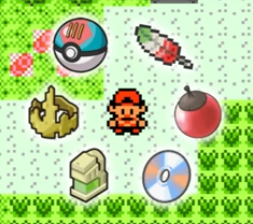
\includegraphics[width=0.25\textwidth]{pokeitems.png}
	
		\[
			\begin{array}{lll}
				\textbf{(7, 28)}, & (6, 22), & (5, 18),\\
				\textbf{(2, 6)}, & (3, 7), & \textbf{(1, 1)}.
			\end{array}
		\]
	If the items are sorted in decreasing order of
	value-to-weight ratio, the greedy algorithm would fill the knapsack with
	items 1, 4 and 6.
\end{frame}

%

\begin{frame}{Knapsack - DP}
	The total value achieved by the greedy algorithm was 35. Can we do better?
	\pause

	\bigskip
	Let the table \textbf{memo} be filled in such a way that \textbf{memo[i,j]}
	is the maximum value that can be carried in a knapsack of capacity
	\textbf{j} and available items 1 to \textbf{i}.

	\bigskip
	\begin{tabular}{|| l|| c|c|c|c|c|c|c|c|c|c|c ||}\hline
		\textbf{j} & 1 & 2 & 3 & 4 & 5  & 6  & 7  & 8  & 9  & 10 & 11\\\hline\hline
		\textbf{i} & x & x & x & x & x  & x  & x  & x  & x  &  x & x\\\hline\hline\pause
		1          & 1 & 1 & 1 & 1 & 1  & 1  & 1  & 1  & 1  &  1 & 1\\\hline\pause
		2          & 1 & 6 & 7 & 7 & 7  & 7  & 7  & 7  & 7  &  7 & 7\\\hline\pause
		3          & 1 & 6 & 7 & 8 & 13 & 14 & 14 & 14 & 14 & 14 & 14\\\hline\pause
		4          & 1 & 6 & 7 & 8 & 18 & 19 & 24 & 25 & 26 & 31 & 32\\\hline\pause
		5          & 1 & 6 & 7 & 8 & 18 & 22 & 24 & 28 & 29 & 31 & 40\\\hline\pause
		6          & 1 & 6 & 7 & 8 & 18 & 22 & 28 & 29 & 34 & 35 & 40\\\hline
	\end{tabular} 
\end{frame}

%

\begin{frame}{Matrix bracketing}
	Matrix multiplication is associative, so given the matrices
	$A \in \Rmat{p}{q}$, $B \in \Rmat{q}{r}$, and $C \in \Rmat{r}{s}$ we have
	two possible bracketings of their product:

	\(
		(AB)C
	\)
	and
	\(
		A(BC)
	\).

	\bigskip
	The cost of computing the row-by-column product $AB$ is $pqr$ (Exercise),
	so the cost of the first bracketing is $pqr + prs$ and that of the second is
	$pqs + qrs$. We prefer whichever is smallest!

	\bigskip
	\textbf{Convention}. The default association will be to the left, so that
	\[
		\begin{array}{l}
			ABC= (AB)C\\
			A(BC)D= (A(BC))D\\
			AB(CD)= (AB)(CD)\\
			\text{etc}\ldots
		\end{array}
	\]
\end{frame}

%

\begin{frame}{Matrix bracketing}
	\begin{exl}
		If $A \in \Rmat{1}{2}$, $B \in \Rmat{2}{3}$, and $C \in \Rmat{3}{1}$,
		what is the cheapest bracketing for their product?
	\end{exl}

	\begin{exl}
		Same question for $A \in \Rmat{3}{2}$, $B \in \Rmat{2}{5}$,
		$C \in \Rmat{5}{1}$, and $D \in \Rmat{1}{4}$.
	\end{exl}
\end{frame}

%

\begin{frame}{Matrix bracketing - DP}
	$A \in \Rmat{3}{2}$, $B \in \Rmat{2}{5}$, $C \in \Rmat{5}{1}$, and
	$D \in \Rmat{1}{4}$. 

	\bigskip
	To use dynamic programming, fill the table \textbf{memo} so that
	\textbf{memo[i][j]} is the number of multiplications required by the
	best bracketing of the product of $M_i, \ldots, M_j$.
\end{frame}

%

\begin{frame}{Matrix bracketing - DP}
	\lstinputlisting[language=Java, firstline= 128, lastline= 132]{Aula09.java}
\end{frame}

%

\begin{frame}{Matrix bracketing - DP}
	\lstinputlisting[language=Java, firstline= 133, lastline= 153]{Aula09.java}
\end{frame}

%

\begin{frame}{Using a memory function - matrix bracketing}
	We introduced dynamic programming as an alternative to inefficient recursive
	algorithms. However, we can make recursive calls and avoid full-depth
	recursion if we update the memory every time we solve a small subproblem:

	\lstinputlisting[language=Java, firstline= 176, lastline= 176]{Aula09.java}
	\lstinputlisting[language=Java, firstline= 182, lastline= 188]{Aula09.java}
\end{frame}

%

\begin{frame}{Using a memory function - matrix bracketing}
	\lstinputlisting[language=Java, firstline= 189, lastline= 200]{Aula09.java}
\end{frame}

%

\begin{frame}{Using a memory function - matrix bracketing}
	And the full problem is solved by a call of the form
	\lstinputlisting[language=Java, firstline= 159, lastline= 168]{Aula09.java}
\end{frame}

%

\begin{frame}{Using a memory function - knapsack}
	The same approach works for solving the knapsack problem. Our memory
	\textbf{mvt} is such that \textbf{mvt[w]} is the maximum value that can be
	carried with weight limit \textbf{w}.

	\lstinputlisting[language=Java, firstline= 81, lastline= 88]{Aula09.java}
\end{frame}

%

\begin{frame}{Using a memory function - knapsack}
	\lstinputlisting[language=Java, firstline= 90, lastline= 105]{Aula09.java}
\end{frame}
\end{document}
